% The Cauchy product: square of partial sums, small triangle k+l<=N, big triangle k+l<=2N. Generated by figs_t0c05.py.
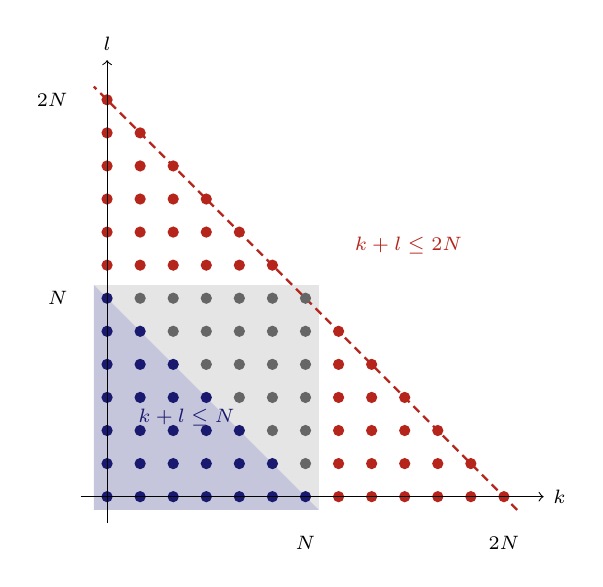
\begin{tikzpicture}[scale=0.42]
\fill[gray!20] (-0.4,-0.4) rectangle (6.4,6.4);
\fill[MidnightBlue!25] (-0.4,-0.4) -- (6.4,-0.4) -- (-0.4,6.4) -- cycle;
\draw[BrickRed,thick,densely dashed] (12.4,-0.4) -- (-0.4,12.4);
\fill[MidnightBlue] (0,0) circle (0.17);
\fill[MidnightBlue] (0,1) circle (0.17);
\fill[MidnightBlue] (0,2) circle (0.17);
\fill[MidnightBlue] (0,3) circle (0.17);
\fill[MidnightBlue] (0,4) circle (0.17);
\fill[MidnightBlue] (0,5) circle (0.17);
\fill[MidnightBlue] (0,6) circle (0.17);
\fill[BrickRed] (0,7) circle (0.17);
\fill[BrickRed] (0,8) circle (0.17);
\fill[BrickRed] (0,9) circle (0.17);
\fill[BrickRed] (0,10) circle (0.17);
\fill[BrickRed] (0,11) circle (0.17);
\fill[BrickRed] (0,12) circle (0.17);
\fill[MidnightBlue] (1,0) circle (0.17);
\fill[MidnightBlue] (1,1) circle (0.17);
\fill[MidnightBlue] (1,2) circle (0.17);
\fill[MidnightBlue] (1,3) circle (0.17);
\fill[MidnightBlue] (1,4) circle (0.17);
\fill[MidnightBlue] (1,5) circle (0.17);
\fill[black!60] (1,6) circle (0.17);
\fill[BrickRed] (1,7) circle (0.17);
\fill[BrickRed] (1,8) circle (0.17);
\fill[BrickRed] (1,9) circle (0.17);
\fill[BrickRed] (1,10) circle (0.17);
\fill[BrickRed] (1,11) circle (0.17);
\fill[MidnightBlue] (2,0) circle (0.17);
\fill[MidnightBlue] (2,1) circle (0.17);
\fill[MidnightBlue] (2,2) circle (0.17);
\fill[MidnightBlue] (2,3) circle (0.17);
\fill[MidnightBlue] (2,4) circle (0.17);
\fill[black!60] (2,5) circle (0.17);
\fill[black!60] (2,6) circle (0.17);
\fill[BrickRed] (2,7) circle (0.17);
\fill[BrickRed] (2,8) circle (0.17);
\fill[BrickRed] (2,9) circle (0.17);
\fill[BrickRed] (2,10) circle (0.17);
\fill[MidnightBlue] (3,0) circle (0.17);
\fill[MidnightBlue] (3,1) circle (0.17);
\fill[MidnightBlue] (3,2) circle (0.17);
\fill[MidnightBlue] (3,3) circle (0.17);
\fill[black!60] (3,4) circle (0.17);
\fill[black!60] (3,5) circle (0.17);
\fill[black!60] (3,6) circle (0.17);
\fill[BrickRed] (3,7) circle (0.17);
\fill[BrickRed] (3,8) circle (0.17);
\fill[BrickRed] (3,9) circle (0.17);
\fill[MidnightBlue] (4,0) circle (0.17);
\fill[MidnightBlue] (4,1) circle (0.17);
\fill[MidnightBlue] (4,2) circle (0.17);
\fill[black!60] (4,3) circle (0.17);
\fill[black!60] (4,4) circle (0.17);
\fill[black!60] (4,5) circle (0.17);
\fill[black!60] (4,6) circle (0.17);
\fill[BrickRed] (4,7) circle (0.17);
\fill[BrickRed] (4,8) circle (0.17);
\fill[MidnightBlue] (5,0) circle (0.17);
\fill[MidnightBlue] (5,1) circle (0.17);
\fill[black!60] (5,2) circle (0.17);
\fill[black!60] (5,3) circle (0.17);
\fill[black!60] (5,4) circle (0.17);
\fill[black!60] (5,5) circle (0.17);
\fill[black!60] (5,6) circle (0.17);
\fill[BrickRed] (5,7) circle (0.17);
\fill[MidnightBlue] (6,0) circle (0.17);
\fill[black!60] (6,1) circle (0.17);
\fill[black!60] (6,2) circle (0.17);
\fill[black!60] (6,3) circle (0.17);
\fill[black!60] (6,4) circle (0.17);
\fill[black!60] (6,5) circle (0.17);
\fill[black!60] (6,6) circle (0.17);
\fill[BrickRed] (7,0) circle (0.17);
\fill[BrickRed] (7,1) circle (0.17);
\fill[BrickRed] (7,2) circle (0.17);
\fill[BrickRed] (7,3) circle (0.17);
\fill[BrickRed] (7,4) circle (0.17);
\fill[BrickRed] (7,5) circle (0.17);
\fill[BrickRed] (8,0) circle (0.17);
\fill[BrickRed] (8,1) circle (0.17);
\fill[BrickRed] (8,2) circle (0.17);
\fill[BrickRed] (8,3) circle (0.17);
\fill[BrickRed] (8,4) circle (0.17);
\fill[BrickRed] (9,0) circle (0.17);
\fill[BrickRed] (9,1) circle (0.17);
\fill[BrickRed] (9,2) circle (0.17);
\fill[BrickRed] (9,3) circle (0.17);
\fill[BrickRed] (10,0) circle (0.17);
\fill[BrickRed] (10,1) circle (0.17);
\fill[BrickRed] (10,2) circle (0.17);
\fill[BrickRed] (11,0) circle (0.17);
\fill[BrickRed] (11,1) circle (0.17);
\fill[BrickRed] (12,0) circle (0.17);
\draw[->] (-0.8,0) -- (13.2,0) node[right,font=\scriptsize] {$k$};
\draw[->] (0,-0.8) -- (0,13.2) node[above,font=\scriptsize] {$l$};
\node[font=\scriptsize,anchor=north] at (6,-0.9) {$N$};
\node[font=\scriptsize,anchor=north] at (12,-0.9) {$2N$};
\node[font=\scriptsize,anchor=east] at (-0.9,6) {$N$};
\node[font=\scriptsize,anchor=east] at (-0.9,12) {$2N$};
\node[font=\scriptsize,MidnightBlue] at (2.4,2.4) {$k+l\le N$};
\node[font=\scriptsize,BrickRed,anchor=west] at (7.2,7.6) {$k+l\le2N$};
\end{tikzpicture}
